\documentclass[lettersize,journal]{IEEEtran}
\usepackage{amsmath,amsfonts}
\usepackage{algorithmic}
\usepackage{algorithm}
\usepackage{array}
\usepackage[caption=false,font=normalsize,labelfont=sf,textfont=sf]{subfig}
\usepackage{textcomp}
\usepackage{stfloats}
\usepackage{url}
\usepackage{verbatim}
\usepackage{graphicx}
\usepackage{cite}
\usepackage{blindtext}
\hyphenation{op-tical net-works semi-conduc-tor IEEE-Xplore}
% updated with editorial comments 8/9/2021

\newcommand*{\shortblindtext}{Lorem ipsum dolor sit amet, consectetuer adipiscing elit. Etiam lobortis facilisis sem. Nullam nec mi et neque pharetra sollicitudin. Praesent imperdiet mi nec ante.}

\newcommand{\paperTitle}{Title}

\begin{document}

\title{\paperTitle}

\author{Theofilos A. Papadopoulos,~\IEEEmembership{Senior Member,~IEEE}, Zacharias G. Datsios,~\IEEEmembership{Member,~IEEE}, Andreas I. Chrysochos,~\IEEEmembership{Member,~IEEE}, Amauri G. Martins-Britto,~\IEEEmembership{Member,~IEEE}, Pantelis N. Mikropoulos,~\IEEEmembership{Senior Member,~IEEE}, and Grigoris K. Papagiannis,~\IEEEmembership{Senior Member,~IEEE}
        % <-this % stops a space
\thanks{Affiliations go here.}% <-this % stops a space
\thanks{Manuscript received mmmm dd, yyyy; revised mmmm dd, yyyy.}}

% The paper headers
\markboth{IEEE TRANSACTIONS ON ELECTROMAGNETIC COMPATIBILITY}%
{Shell \MakeLowercase{\textit{et al.}}: \paperTitle}

%\IEEEpubid{0000--0000/00\$00.00~\copyright~2021 IEEE}
% Remember, if you use this you must call \IEEEpubidadjcol in the second
% column for its text to clear the IEEEpubid mark.

\maketitle

\begin{abstract}
\shortblindtext
\end{abstract}

\begin{IEEEkeywords}
Earth conduction effects, electromagnetic transients, frequency-dependent soil models, overhead lines.
\end{IEEEkeywords}

\section{Introduction}
%\IEEEPARstart{T}{his} 
\shortblindtext 

\section{Mathematical model}

\subsection{Earth impedance and admittance formulas}
\shortblindtext

\subsection{Frequency-dependent soil model}
\shortblindtext

\section{Propagation characteristics}

\subsection{System configuration}
\shortblindtext

\subsection{Modal analysis}

\shortblindtext
\begin{figure}[tbh]
	\centering
	\label{fig:CharImped_FD0_Ztot_Wise_Ytot_Wise_rho1000_eps5}
	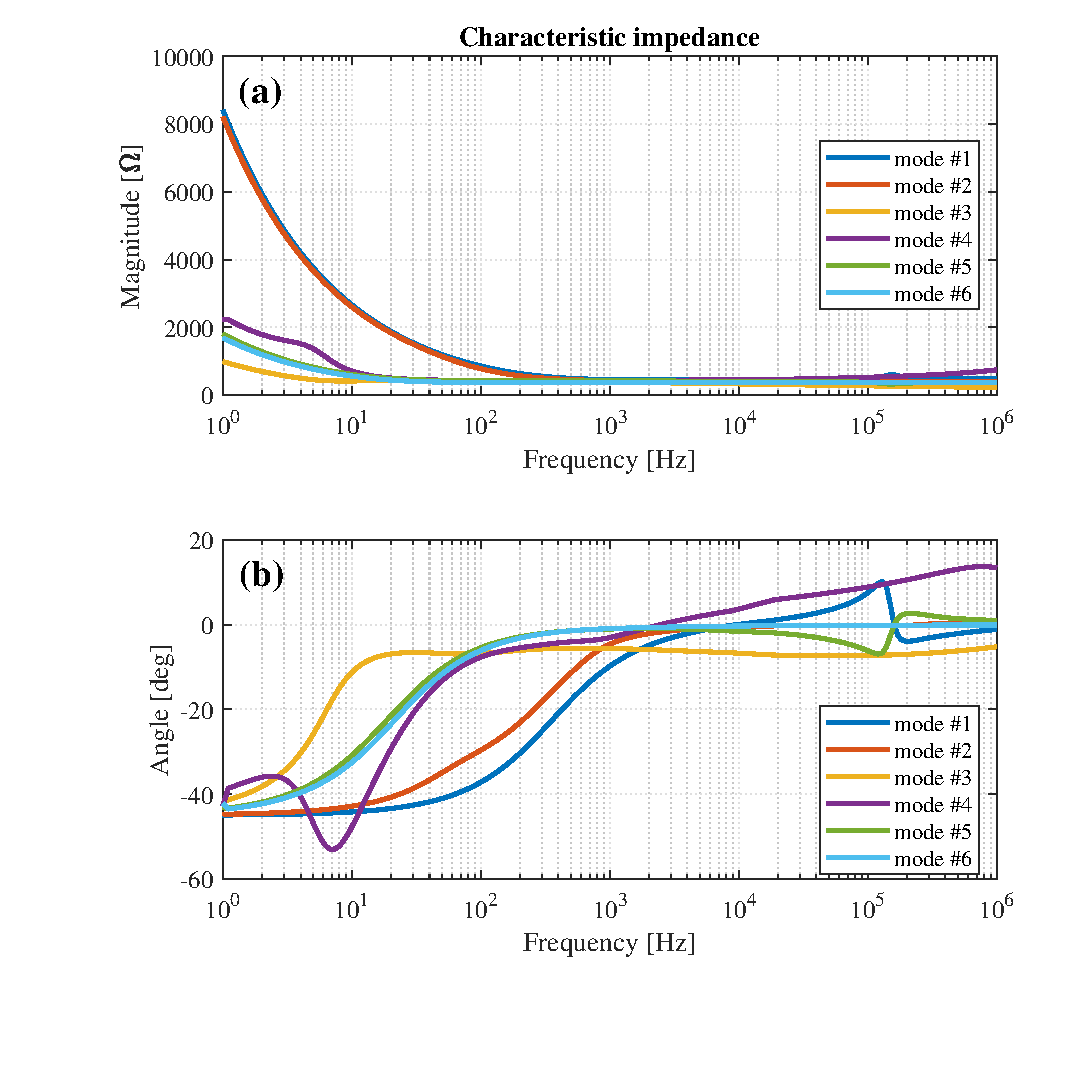
\includegraphics[width=1\columnwidth]{./fig/CharImped_FD0_Ztot_Wise_Ytot_Wise_rho1000_eps5.eps}
	\caption{Characteristic impedance magnitude (a) and angle (b), Wise's formula, constant soil parameters with $\rho = 1000 \: \Omega$.m.}
\end{figure}

\shortblindtext
\begin{figure}[tbh]
	\centering
	\label{fig:AtnConst_PhaseVel_FD0_Ztot_Wise_Ytot_Wise_rho1000_eps5}
	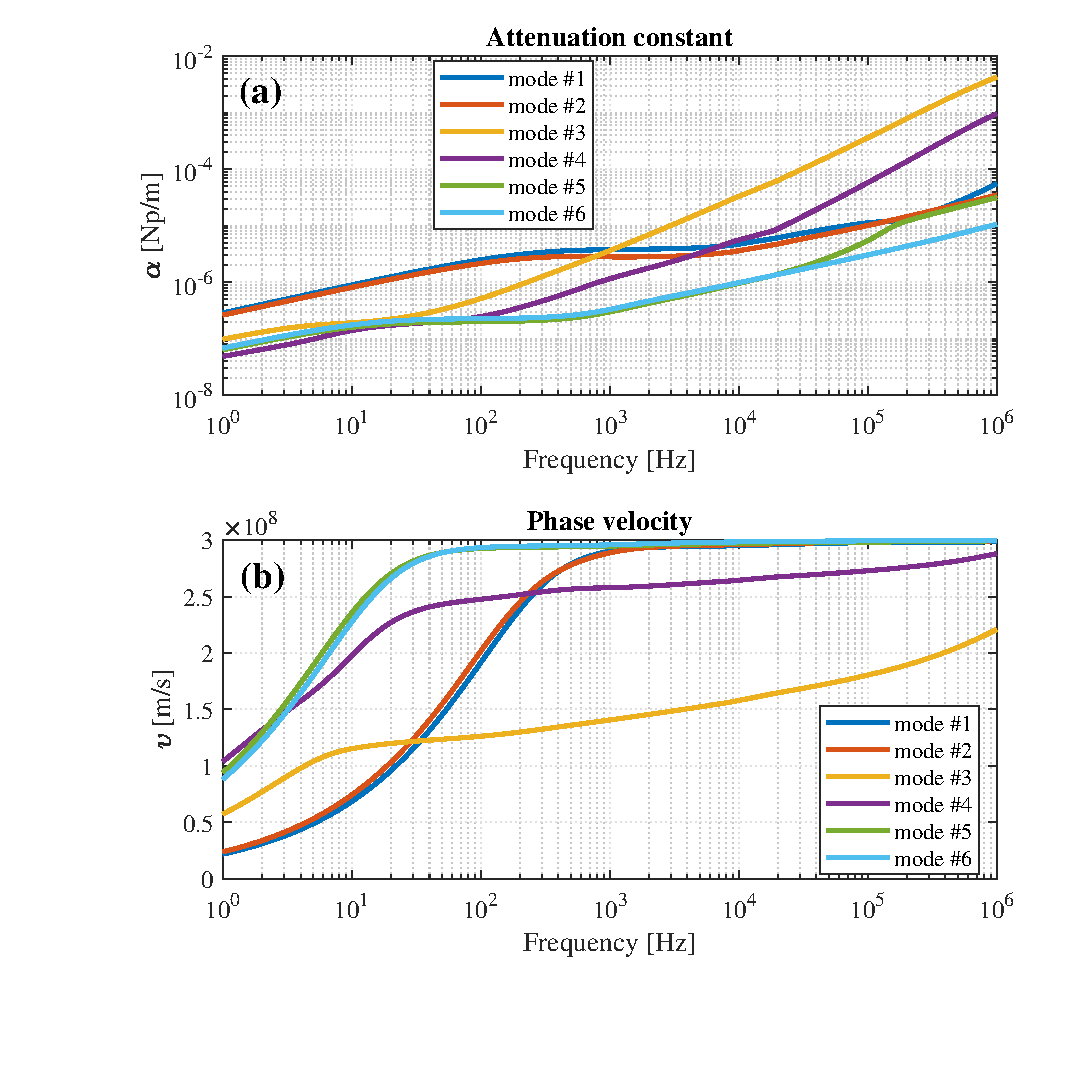
\includegraphics[width=1\columnwidth]{./fig/AtnConst_PhaseVel_FD0_Ztot_Wise_Ytot_Wise_rho1000_eps5.eps}
	\caption{Attenuation constant (a) and phase velocity (b), Wise's formula, constant soil parameters with $\rho = 1000 \: \Omega$.m.}
\end{figure}

\shortblindtext
\onecolumn
\begin{figure}[tbh]
	\centering
	\label{fig:TransfMat_FD0_Ztot_Wise_Ytot_Wise_rho1000_eps5}
	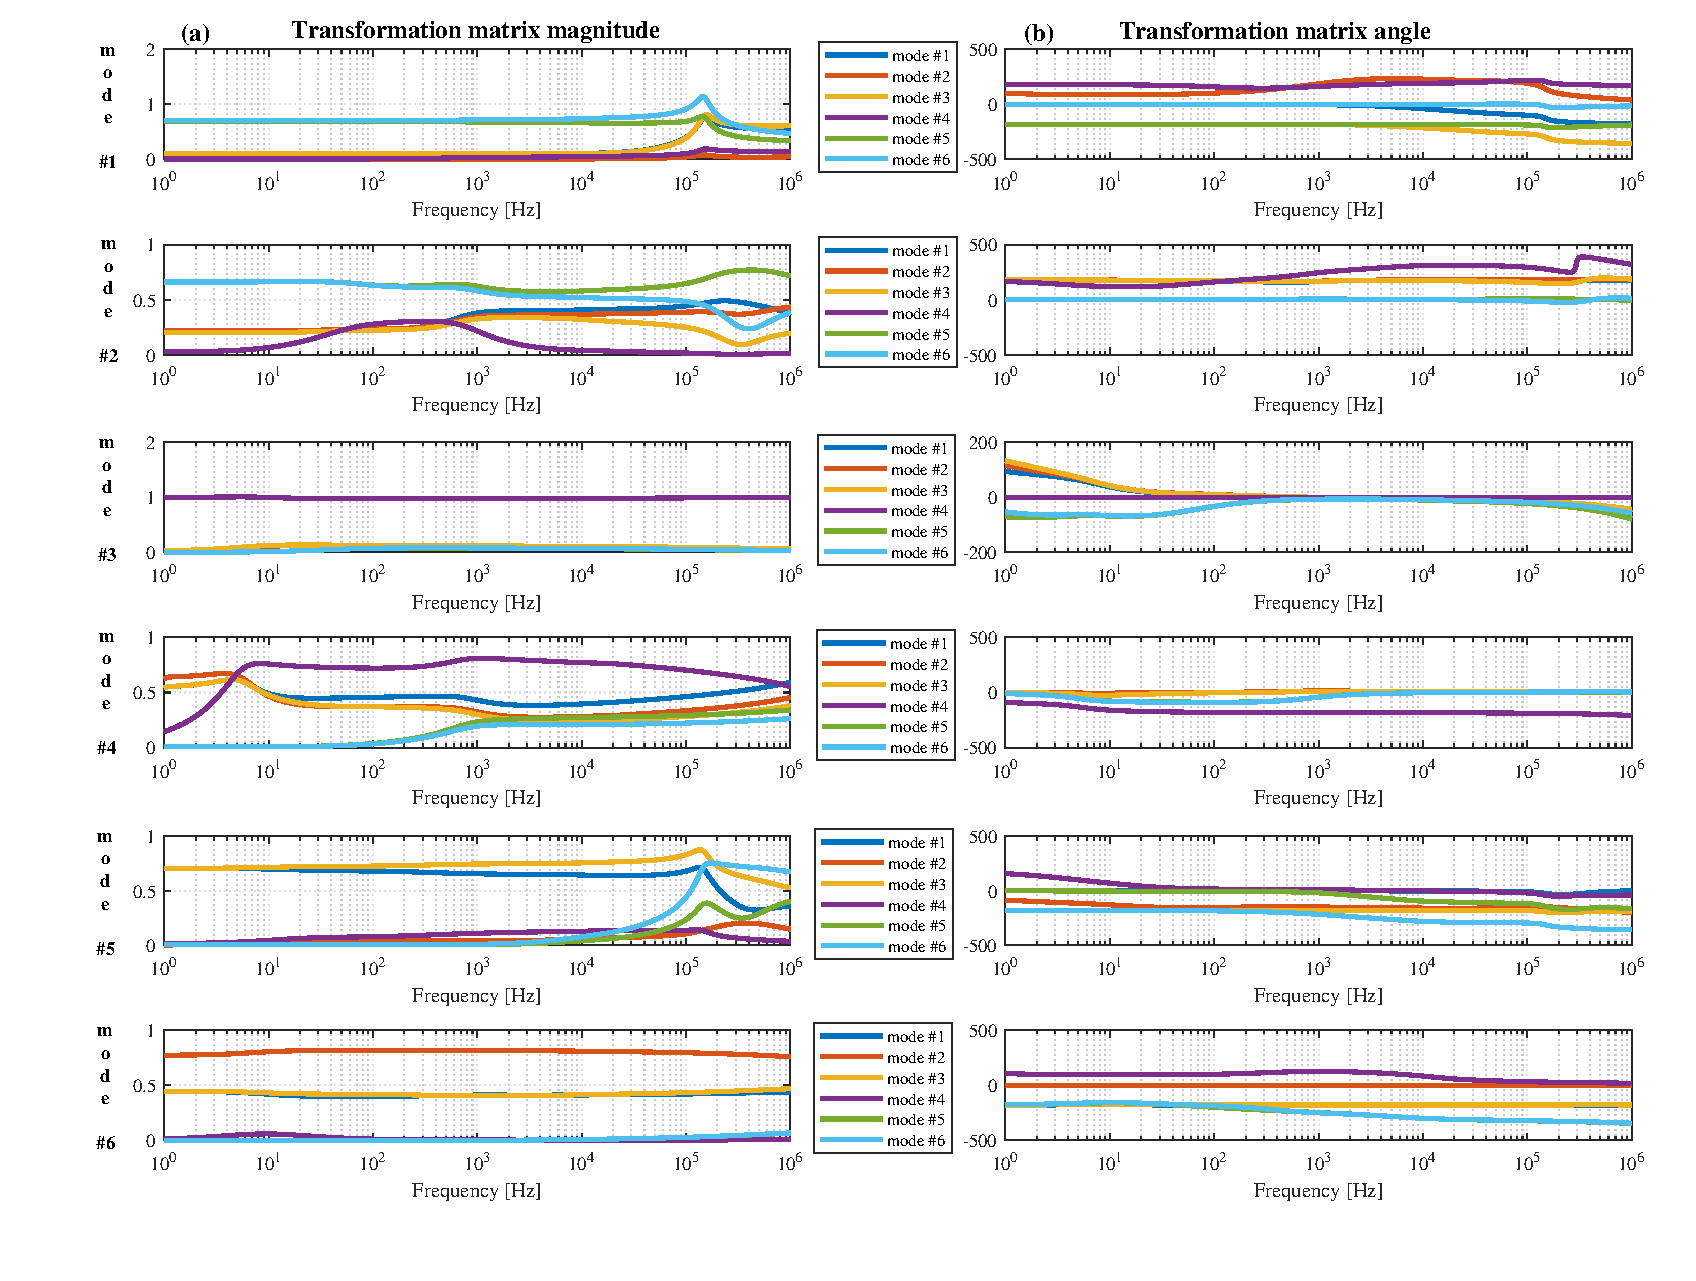
\includegraphics[width=1\columnwidth]{./fig/TransfMat_FD0_Ztot_Wise_Ytot_Wise_rho1000_eps5.eps}
%	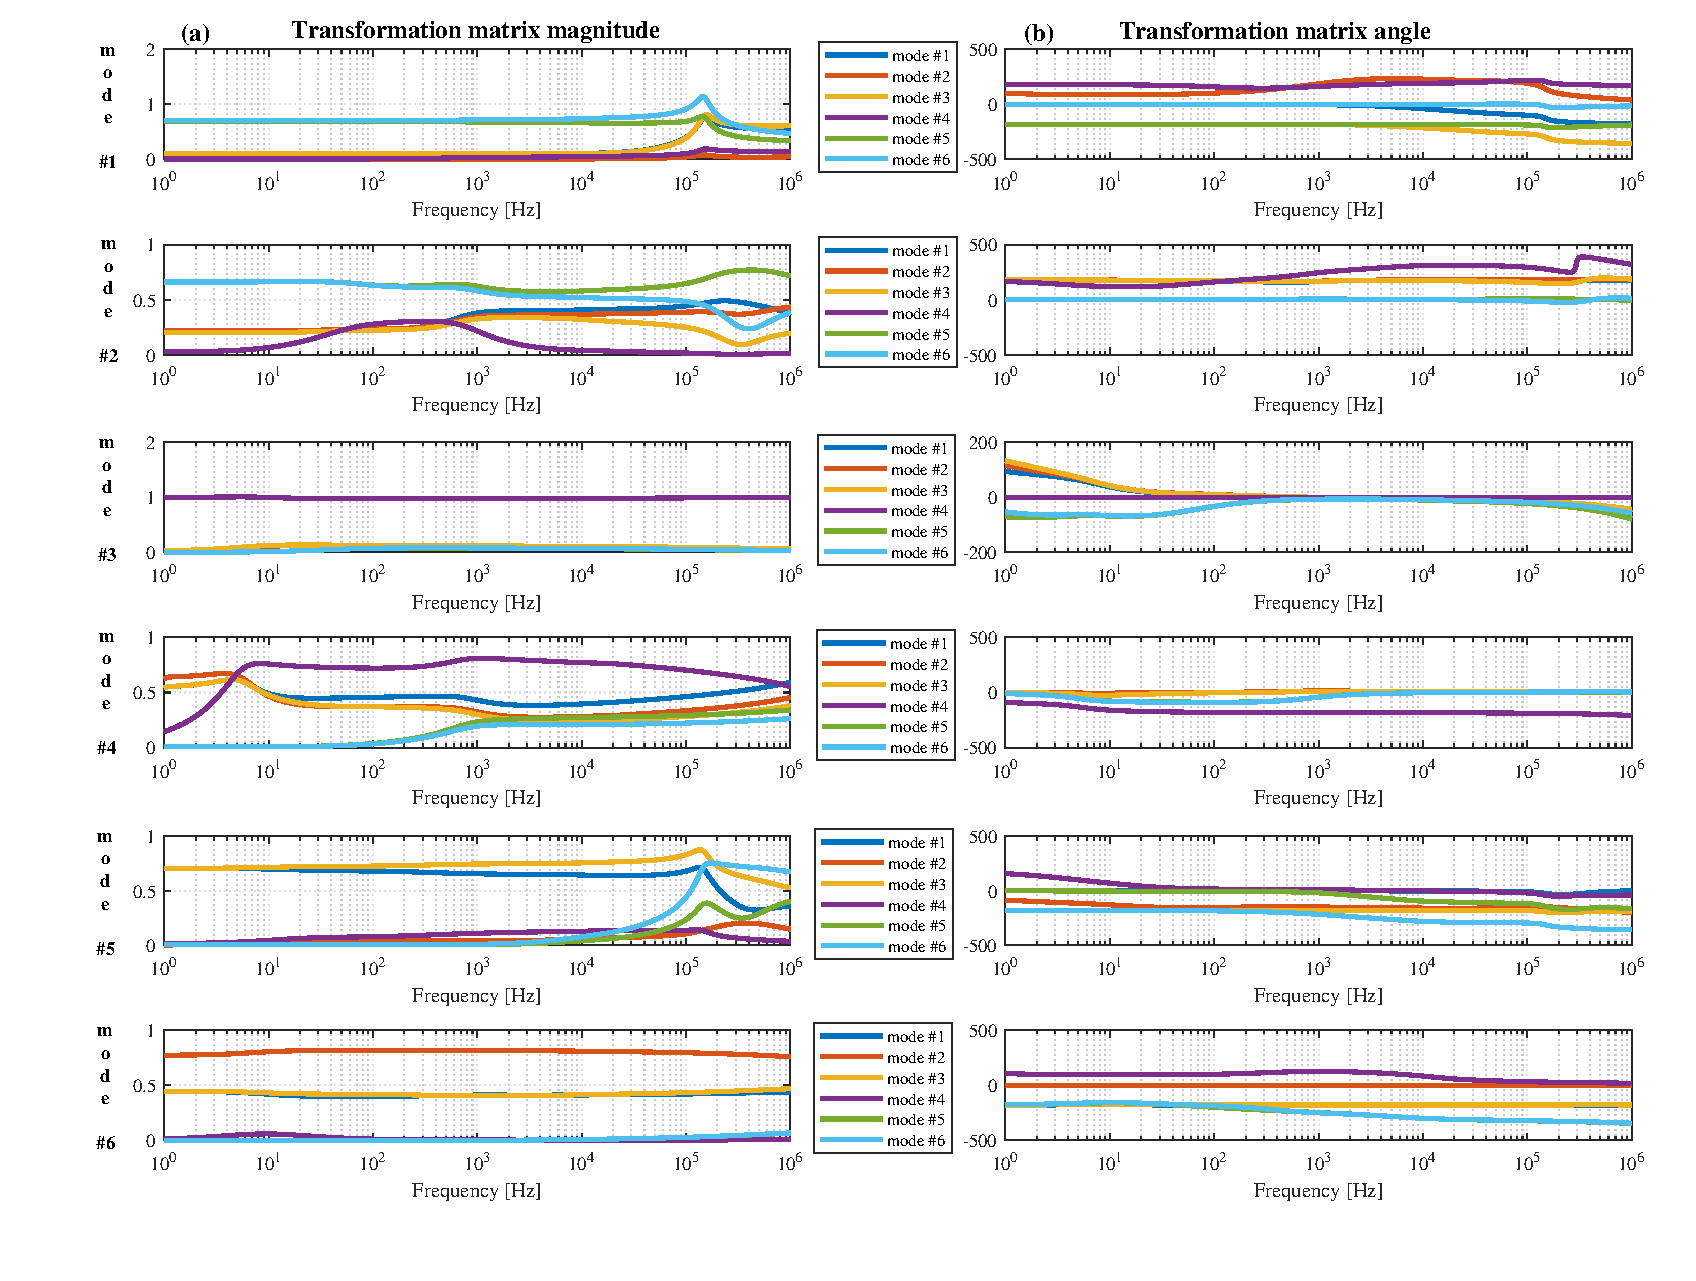
\includegraphics[width=516pt]{./fig/TransfMat_FD0_Ztot_Wise_Ytot_Wise_rho1000_eps5.eps}
	\caption{Modal transformation matrix magnitude  (a) and angle in degrees (b), Wise's formula, constant soil parameters with $\rho = 1000 \: \Omega$.m.}
\end{figure}
\twocolumn

\subsection{Influence of earth admittance correction}

\shortblindtext
\begin{figure}[ht]
	\centering
	\label{fig:WisCarPropag_noratio___const_model_mode3}
	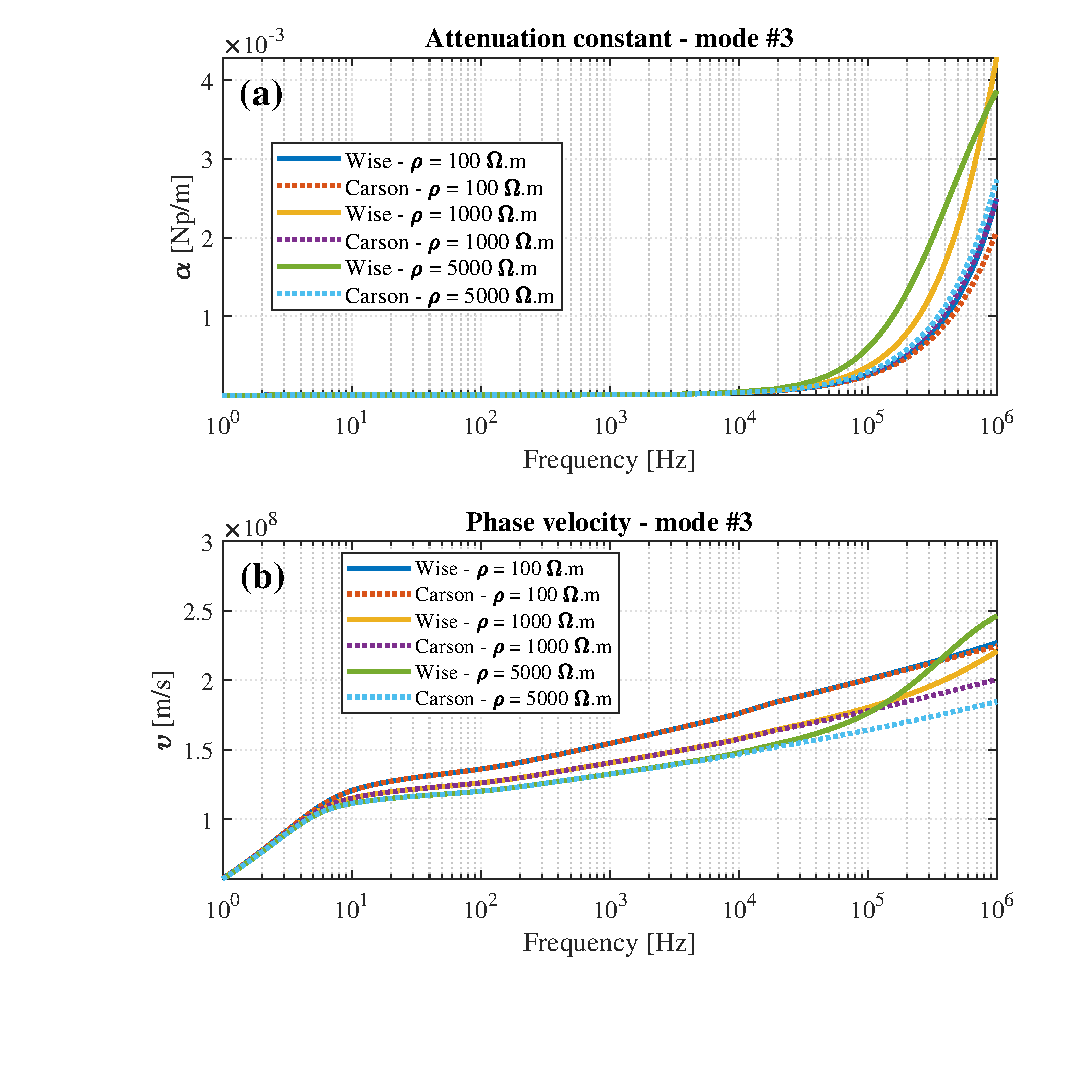
\includegraphics[width=1\columnwidth]{./fig/WisCarPropag_noratio___const_model_mode3.eps}
	\caption{Attenuation constant (a) and phase velocity (b) for mode \#3 (ground mode), comparing Carson and Wise's admittance formulas, with constant soil parameters and different soil resistivities.}
\end{figure}

\shortblindtext
\begin{figure}[ht]
	\centering
	\label{fig:WiseCarson___rho___CP_mode3}
	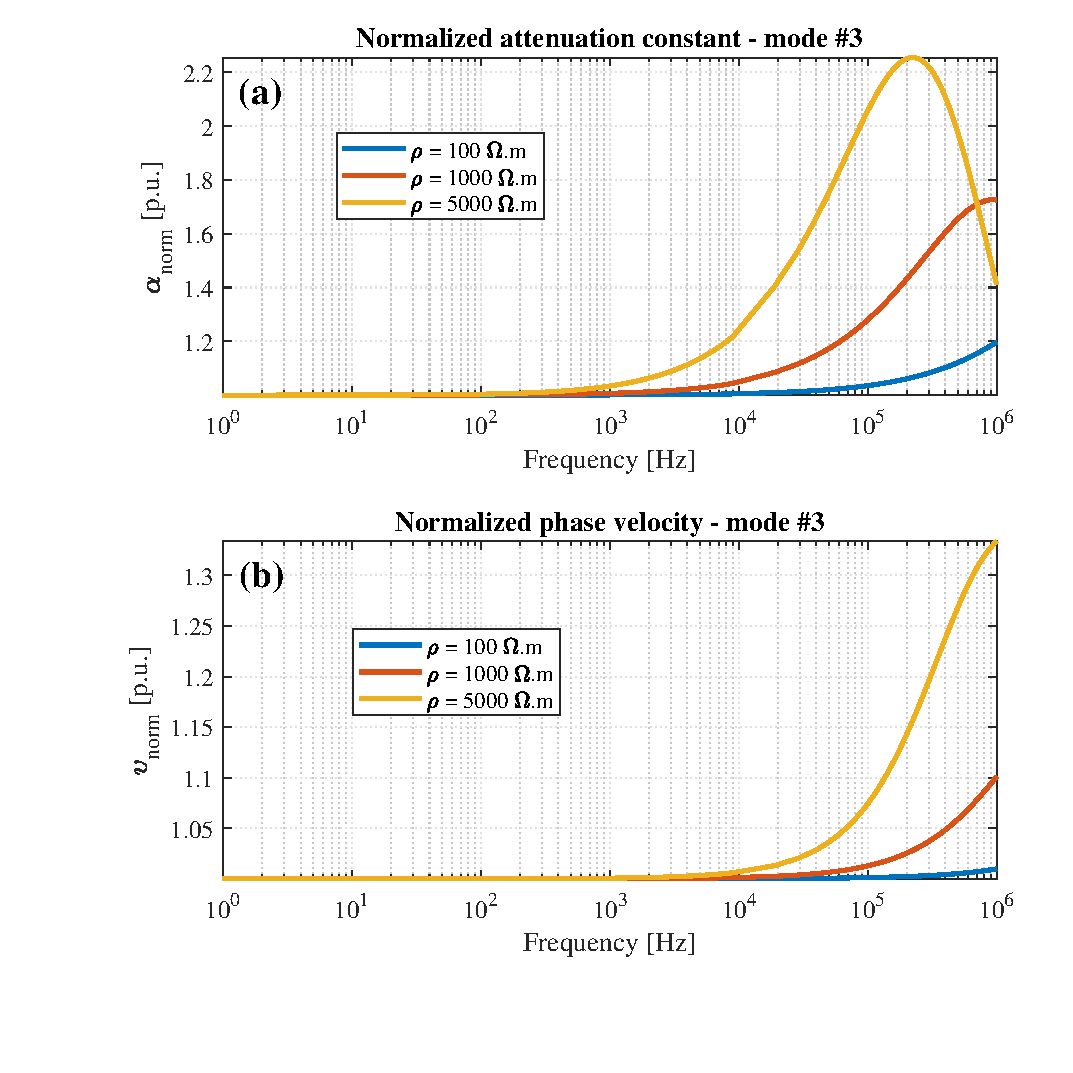
\includegraphics[width=1\columnwidth]{./fig/WiseCarson___rho___CP_mode3.eps}
	\caption{Normalized attenuation constant (a) and phase velocity (b) for mode \#3 (ground mode), comparing Carson and Wise's admittance formulas, with constant soil parameters and different soil resistivities.}
\end{figure}

\shortblindtext
\begin{figure}[tbh]
	\centering
	\label{fig:WisCarPropag_noratio___const_model_mode4}
	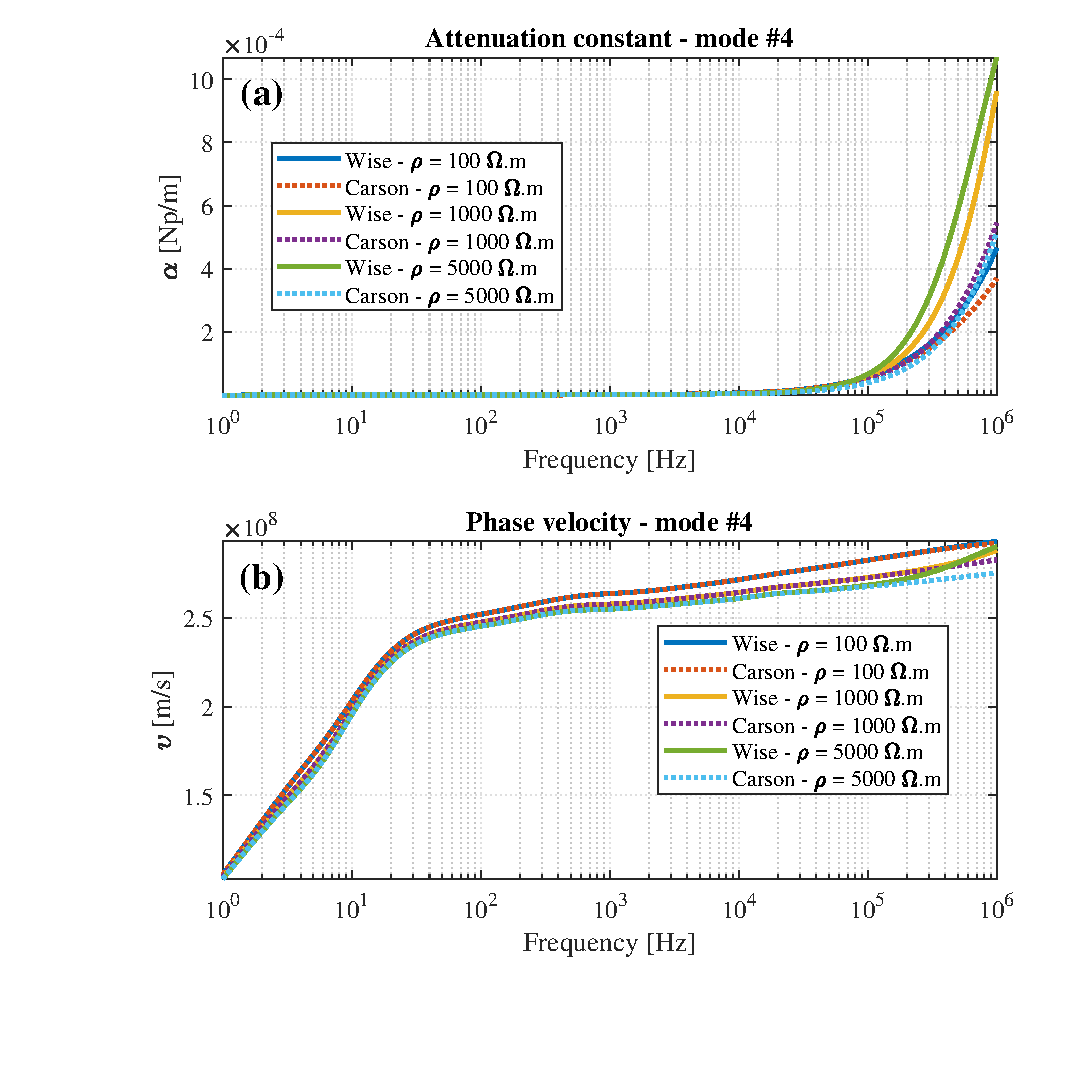
\includegraphics[width=1\columnwidth]{./fig/WisCarPropag_noratio___const_model_mode4.eps}
	\caption{Attenuation constant (a) and phase velocity (b) for mode \#4 (pipeline mode), comparing Carson and Wise's admittance formulas, with constant soil parameters and different soil resistivities.}
\end{figure}

\shortblindtext
\begin{figure}[tbh]
	\centering
	\label{fig:WiseCarson___rho___CP_mode4}
	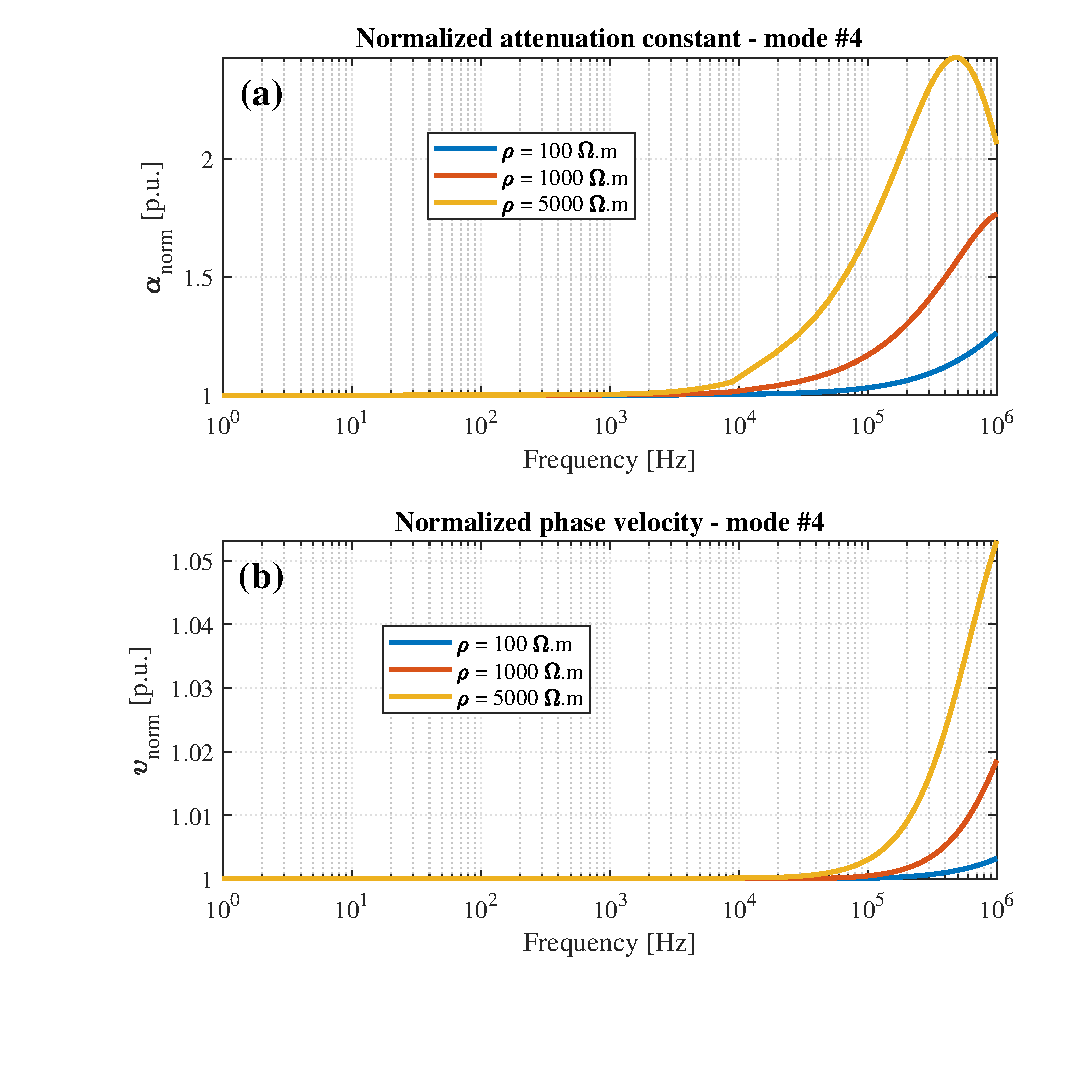
\includegraphics[width=1\columnwidth]{./fig/WiseCarson___rho___CP_mode4.eps}
	\caption{Normalized attenuation constant (a) and phase velocity (b) for mode \#4 (pipeline mode), comparing Carson and Wise's admittance formulas, with constant soil parameters and different soil resistivities.}
\end{figure}

\subsection{Influence of soil model}
\shortblindtext
\begin{figure}[tbh]
	\centering
	\label{fig:WiSoilModel_ratio_mode3}
	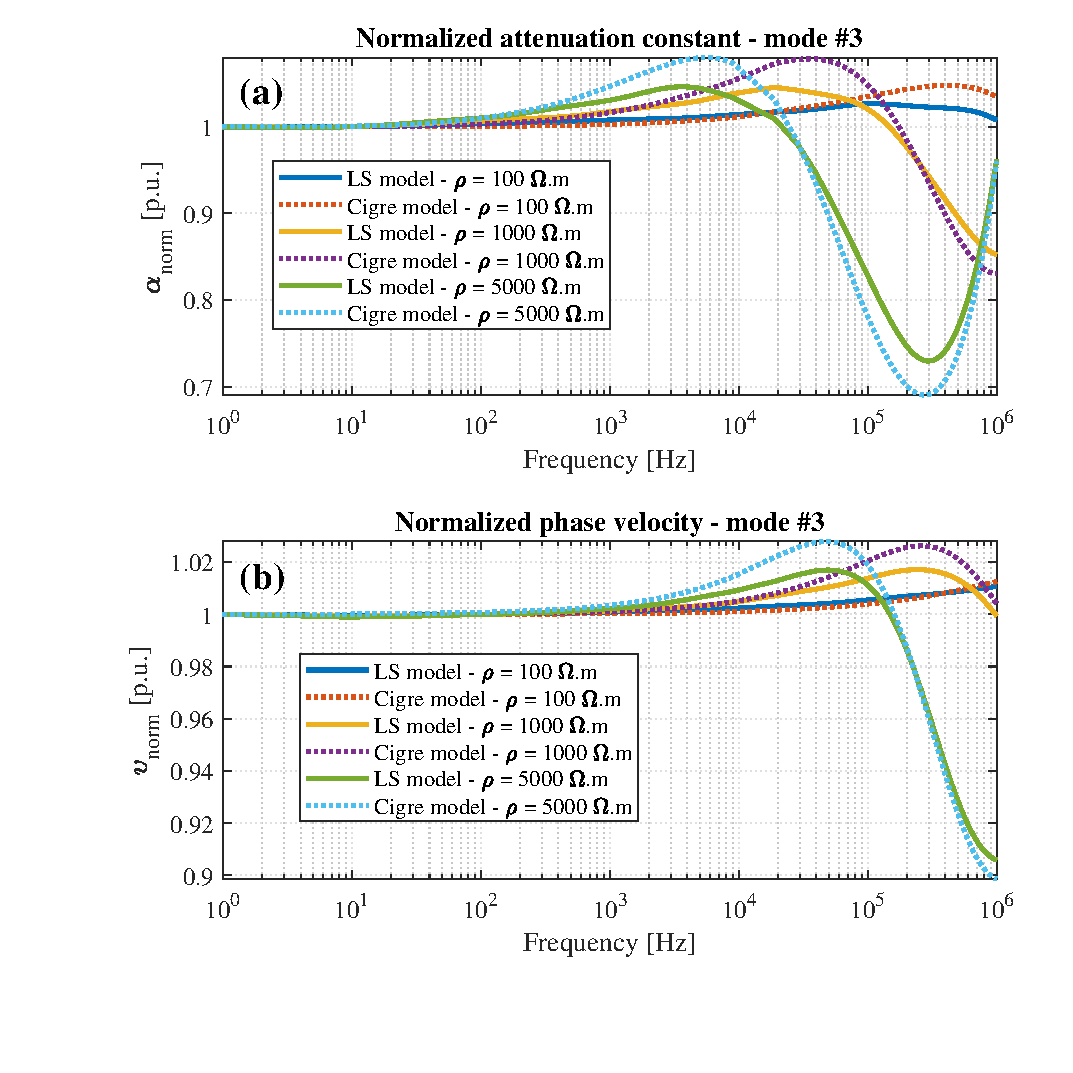
\includegraphics[width=1\columnwidth]{./fig/WiSoilModel_ratio_mode3.eps}
	\caption{Normalized attenuation constant (a) and phase velocity (b) for mode \#3 (ground mode), comparing LS and Cigre frequency-dependence models, using Wise's formula and different soil resistivities.}
\end{figure}

\shortblindtext
\begin{figure}[tbh]
	\centering
	\label{fig:WiSoilModel_ratio_mode4}
	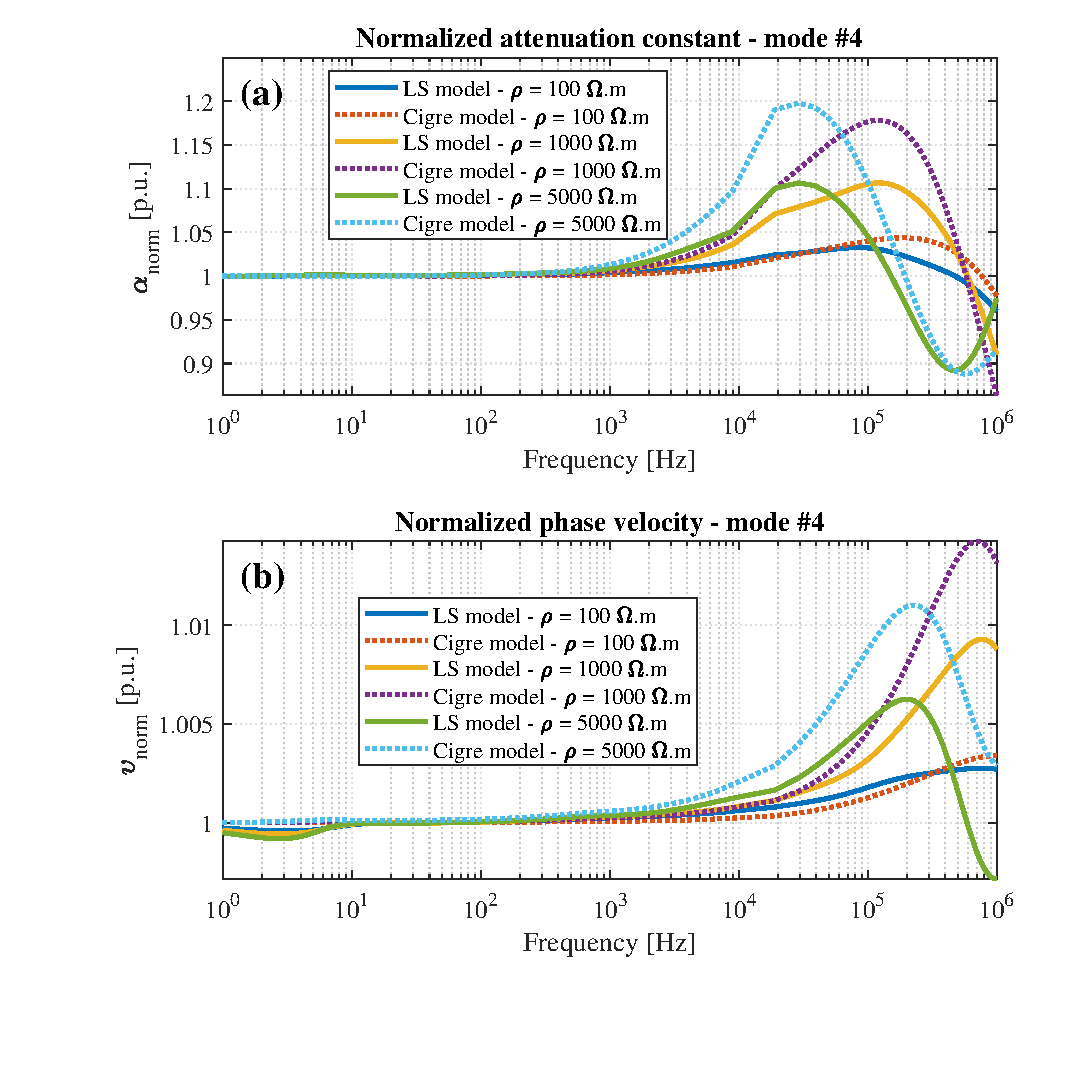
\includegraphics[width=1\columnwidth]{./fig/WiSoilModel_ratio_mode4.eps}
	\caption{Normalized attenuation constant (a) and phase velocity (b) for mode \#4 (pipeline mode), comparing LS and Cigre frequency-dependence models, using Wise's formula and different soil resistivities.}
\end{figure}

\section{Pipeline induced voltages}

\subsection{Frequency-domain responses}
\shortblindtext

\subsection{Transient responses}
\shortblindtext

\section{Conclusions}
\shortblindtext

\section*{Acknowledgments}
\shortblindtext





%{\appendices
%\section*{Proof of the First Zonklar Equation}
%Appendix one text goes here.
% You can choose not to have a title for an appendix if you want by leaving the argument blank
%\section*{Proof of the Second Zonklar Equation}
%Appendix two text goes here.}


\begin{thebibliography}{1}
\bibliographystyle{IEEEtran}

\bibitem{ref1}
{\it{Bibliography goes here}}.

\end{thebibliography}


%\newpage

%\section{Biography Section}
%If you have an EPS/PDF photo (graphicx package needed), extra braces are
% needed around the contents of the optional argument to biography to prevent
 %the LaTeX parser from getting confused when it sees the complicated
 %$\backslash${\tt{includegraphics}} command within an optional argument. (You can create
 %your own custom macro containing the $\backslash${\tt{includegraphics}} command to make things
 %simpler here.)
 
%\vspace{11pt}

%\bf{If you include a photo:}\vspace{-33pt}
%\begin{IEEEbiography}[{\includegraphics[width=1in,height=1.25in,clip,keepas%pectratio]{fig1}}]{Michael Shell}
%Use $\backslash${\tt{begin\{IEEEbiography\}}} and then for the 1st %argument use $\backslash${\tt{includegraphics}} to declare and link the %author photo.
%Use the author name as the 3rd argument followed by the biography text.
%\end{IEEEbiography}

%\vspace{11pt}

%\bf{If you will not include a photo:}\vspace{-33pt}
%\begin{IEEEbiographynophoto}{John Doe}
%Use $\backslash${\tt{begin\{IEEEbiographynophoto\}}} and the author name %as the argument followed by the biography text.
%\end{IEEEbiographynophoto}




\vfill

\end{document}


